\label{sec:query_performance_analysis}

This section evaluates the effectiveness of the solution over the ability to recommend optimizer configurations and improve query runtime as a result. It starts with a predictive model comparison between different types of algorithms and the feasibility of using deep learning approaches in this type of problem. It then evaluates whether the machine learning-based approach can improve the overall query runtime or not compared to the query optimizer by itself.

For every experiment that considers the greedy enumeration algorithm described in the previous chapter, the arbitrary number \textit{m} that defines the initial configuration size was set to a default value of 2.

\subsection{Predictive Model Comparison}

One of the key goals of the experiments was to evaluate the effectiveness of different types of machine learning algorithms to predict query runtime. This comparison is based on how well the different predictive models could be employed in the configuration selection algorithm and observe to what extent they could improve the overall query performance.

\subsubsection{Traditional Algorithms}

Initially, the Random Forest and Support Vector Regression models were evaluated, while treating the problem as a regression task. The Linear Regression model was discarded altogether due to low accuracy during the model validation phase.

\begin{figure}[H]
  \begin{subfigure}[t]{0.5\textwidth}
    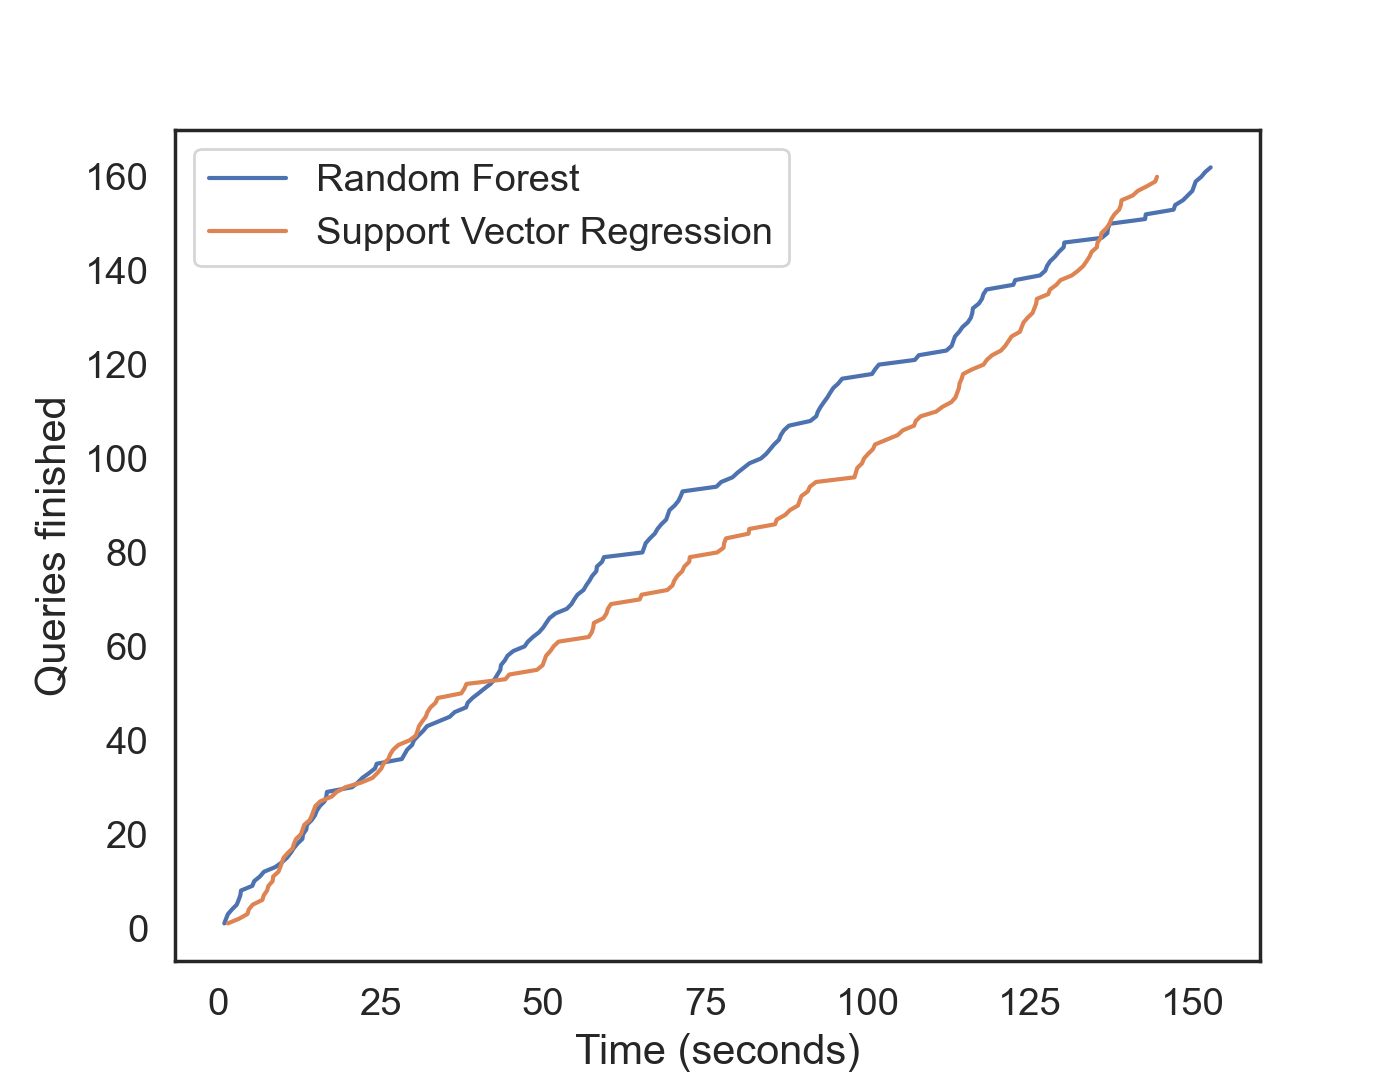
\includegraphics[width=\textwidth]{img/performance_evaluation/tpch_models_comparison.png}
    \caption{\gls{tpch} workload}
  \end{subfigure}\hfill
  \begin{subfigure}[t]{0.5\textwidth}
    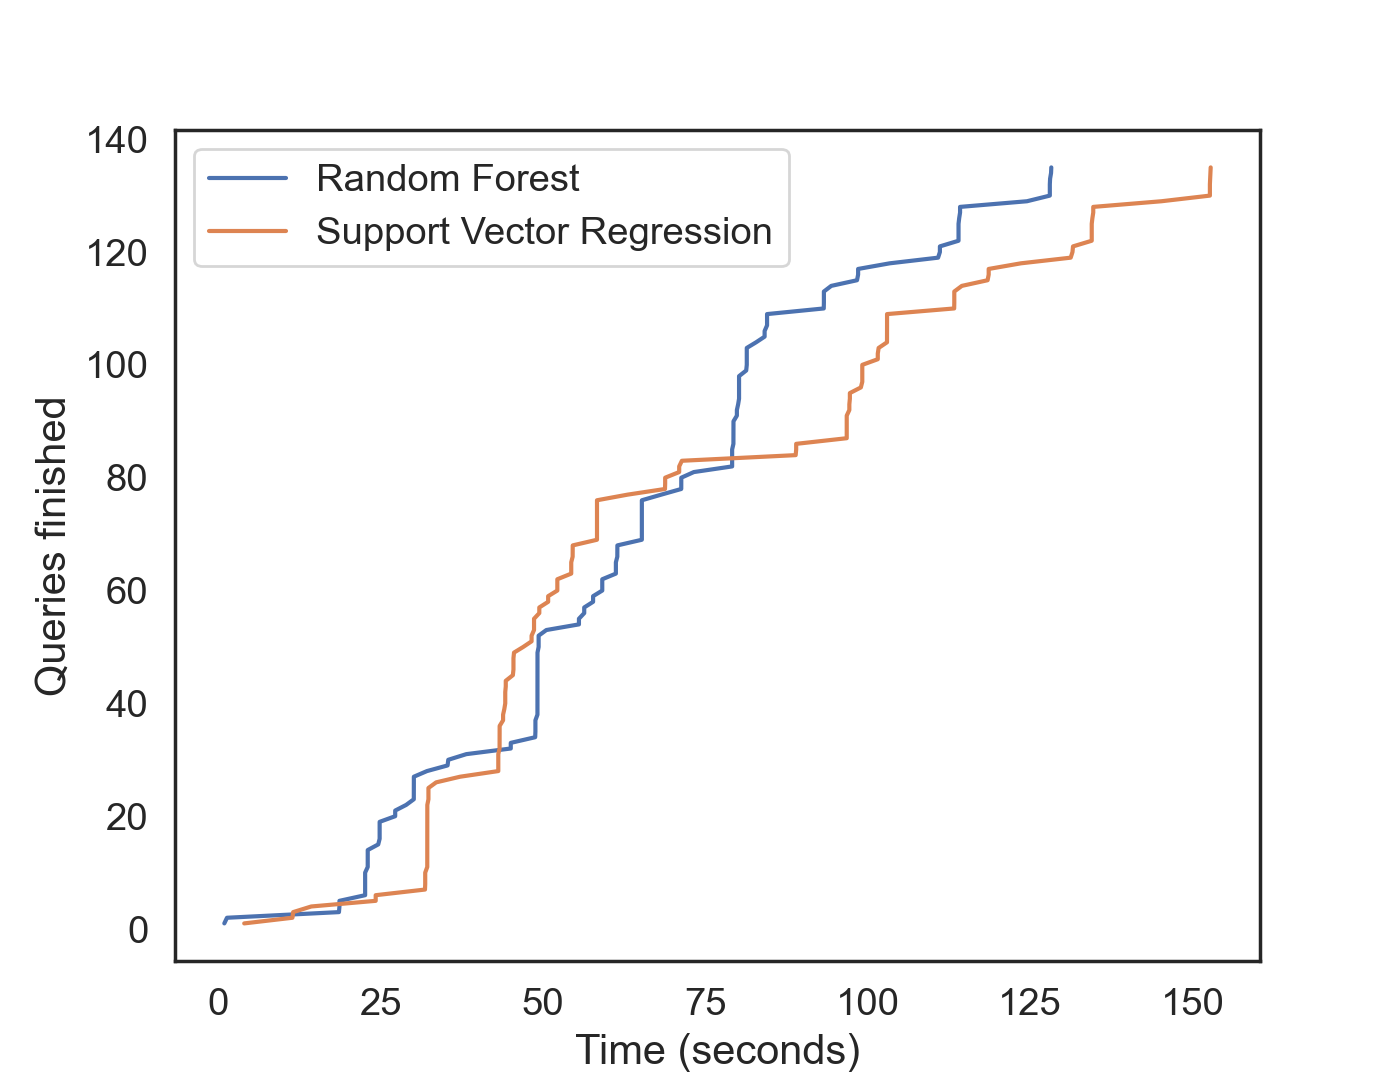
\includegraphics[width=\textwidth]{img/performance_evaluation/job_models_comparison.png}
    \caption{\gls{job} workload}
  \end{subfigure}
  \caption{Traditional predictive model comparison for the \gls{tpch} and \gls{job} workloads}
  \label{fig:model_comparison}
\end{figure}

Figure \ref{fig:model_comparison} presents a quantitative comparison between the two. Each plot shows the performance curves for the \gls{tpch} workload and the JOB workload. They represent the overall query runtime over a set of queries that were not part of the training data set. It is possible to observe that, for the \gls{tpch} workload, Support Vector Regression outperforms the Random Forest model in the overall execution runtime even though the runtime of the latter flowed at a steadier pace over time. For the \gls{job} workload, Random Forest outperforms Support Vector Regression, meaning that it made better execution plan choices for a short sample of queries, resulting in a meaningful reduction in the overall execution runtime.

\subsubsection{Tree Convolutional Neural Networks}

Even though the two algorithms mentioned above can offer more interpretability and simplicity, in certain scenarios, deep neural networks can increase adaptability at the cost of needing more quality and quantity of data. To determine if this was the case, further experiments were carried out using specialized tree convolutional neural networks.

\begin{figure}[H]
\centering
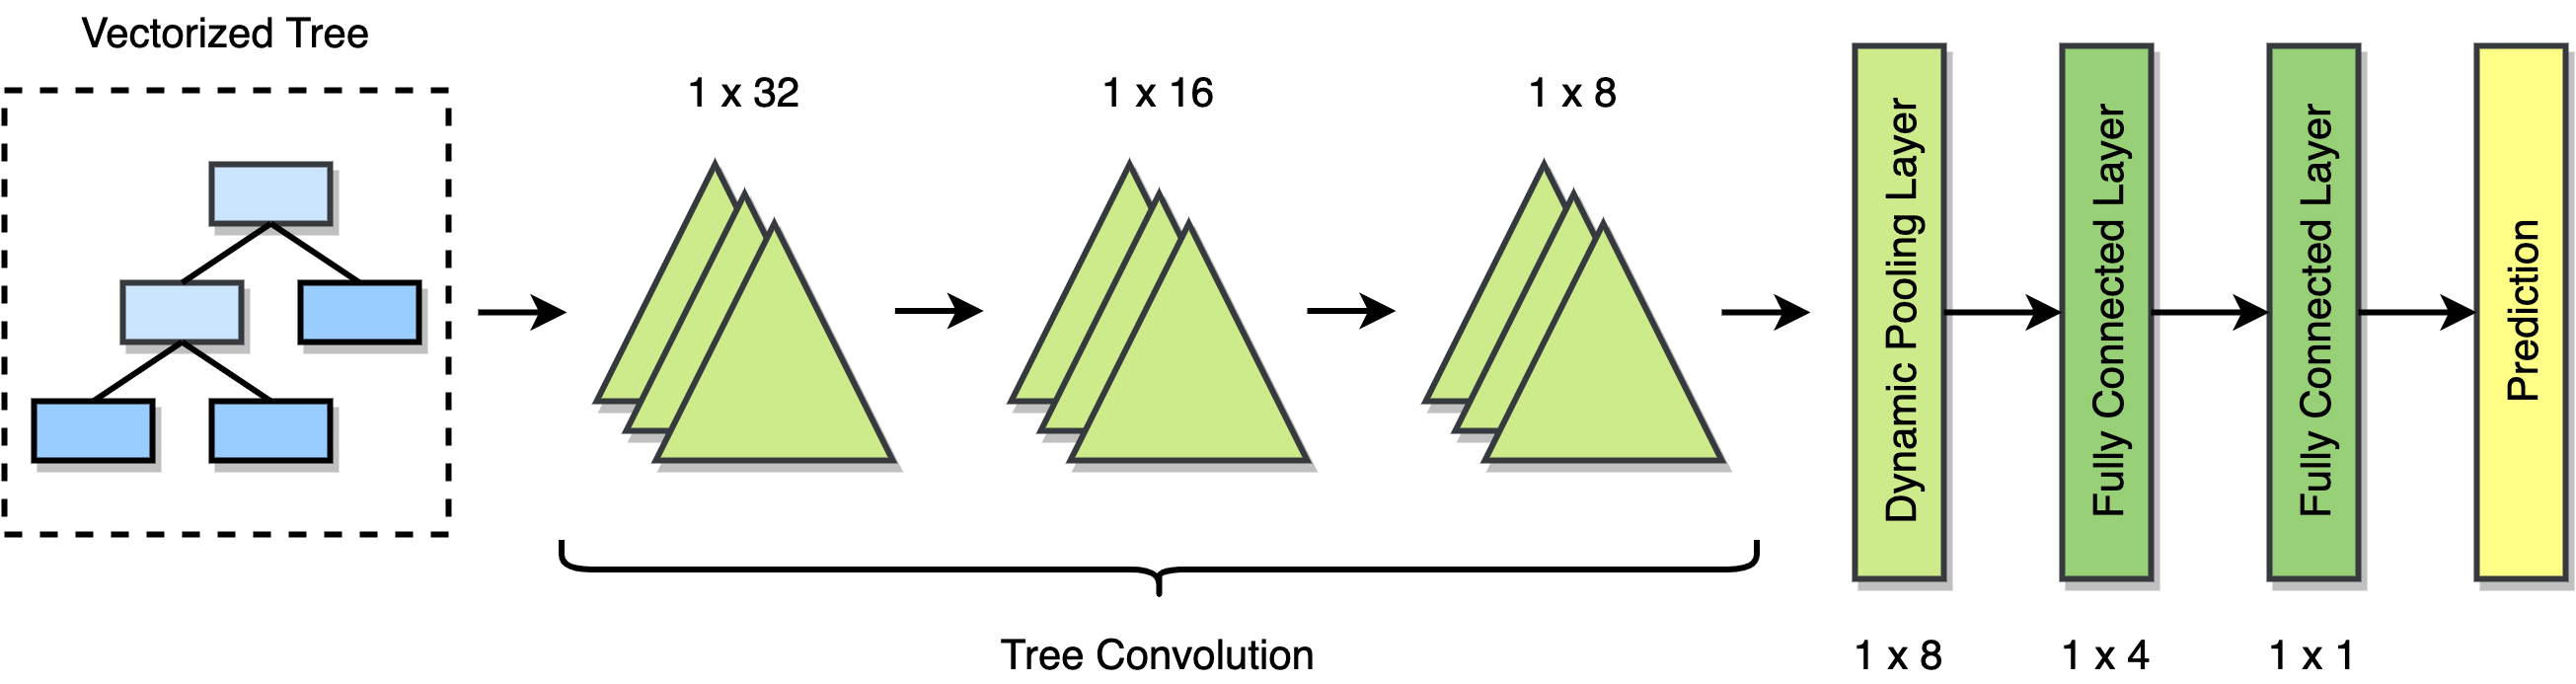
\includegraphics[width=\textwidth]{img/performance_evaluation/tcnn_architecture.png}
\caption{Tree convolutional neural network experimental architecture}
\label{fig:tcnn_experimental_architecture}
\end{figure}

As shown in Figure \ref{fig:tcnn_experimental_architecture}, the used architecture employs three layers of tree convolution, with output dimensions (32, 16, 8), followed by a dynamic pooling layer and two linear layers with output dimensions (4, 1). The Rectified Linear Unit (ReLU) activation functions and layer normalization between each layer were considered. Training is performed with SGD and is ran until 100 epochs elapsed.

To begin with, in contrast to the previous experiments with more traditional algorithms, the number of queries generated per template was increased for the \gls{tpch} workload. Increasing the number of queries per template from 10 to 40, making almost 800 queries would make the training process more robust.

\begin{table}[H]
\centering
\begin{tabular*}{0.5\textwidth}{p{0.25\textwidth} p{0.25\textwidth}}
\hline
\textbf{Batch Size}              & \textbf{\gls{rmse} (ms)}  \\ \hline
4                                & 91 796                   \\
8                                & 93 678                   \\
16                               & 94 099                   \\ \hline
\end{tabular*}
\caption{\gls{rmse} for different batch sizes}
\label{tab:tcnn_results_1}
\end{table}

Table \ref{tab:tcnn_results_1} shows the training results of different batch sizes after 100 epochs elapsed. Even though the training process flowed at a nice and steady pace, the final \gls{rmse}s are not satisfactory. At this point, it is worth considering whether increasing the original data set could lead to better results and proceeded with two additional experiments, which would be done separately:

\begin{itemize}
    \item Increase the database size from 10 GB to 25 GB and evaluate its impact in training;
    \item Double the number of queries per template from 40 to 80 to increase the size of the data set.
\end{itemize}

\begin{table}[H]
\centering
\begin{tabular*}{0.8\textwidth}{p{0.4\textwidth} p{0.4\textwidth}}
\hline
\textbf{Scenario}                & \textbf{Average \gls{rmse} (ms)}  \\ \hline
Scaled-up database of 25 GB      & 394 672                     \\
80 queries per template                   & 84 401                      \\ \hline
\end{tabular*}
\caption{\gls{rmse} for different scenarios during \gls{tcnn} training}
\label{tab:tcnn_results_2}
\end{table}

As shown in Table \ref{tab:tcnn_results_2}, the results with the new scaled-up database were not much different. While it was expectable that the average query runtime would be higher (i.e., 539 331 ms), the average \gls{rmse} was also higher than desirable (i.e., 394 672 ms) in comparison.

For the second experiment, doubling the number of queries per template from 40 to 80 resulted in slightly better results. The average \gls{rmse} of 84 401 ms roughly translates into a decrease of almost 10 seconds in comparison to the experiment with a smaller data set. This leads to conclude that increasing the number of queries per template would help to achieve better results. However, the cost of generating a more extensive data set would be impractical in real-world scenarios.

\subsection{Optimizer Comparison}

Going into more detail in the experimental campaign, the Random Forest model performance was evaluated against the out-of-the-box PostgreSQL query optimizer. With this in mind, a comparison against two different baselines was considered:

\begin{itemize}
    \item The first one refers to the default optimizer configuration where the PostgreSQL optimizer has all settings enabled by default;
    \item The second one represents the enumeration algorithm that makes decisions directly based on cost estimates returned by the optimizer's cost model in contrast to the learned solution that makes its decisions based on the Random Forest model predictions.
\end{itemize}

The idea was to infer whether the same results could be obtained and discard the overhead of collecting execution data and train a machine learning model entirely.

\begin{figure}[H]
    \begin{subfigure}[t]{0.5\textwidth}
    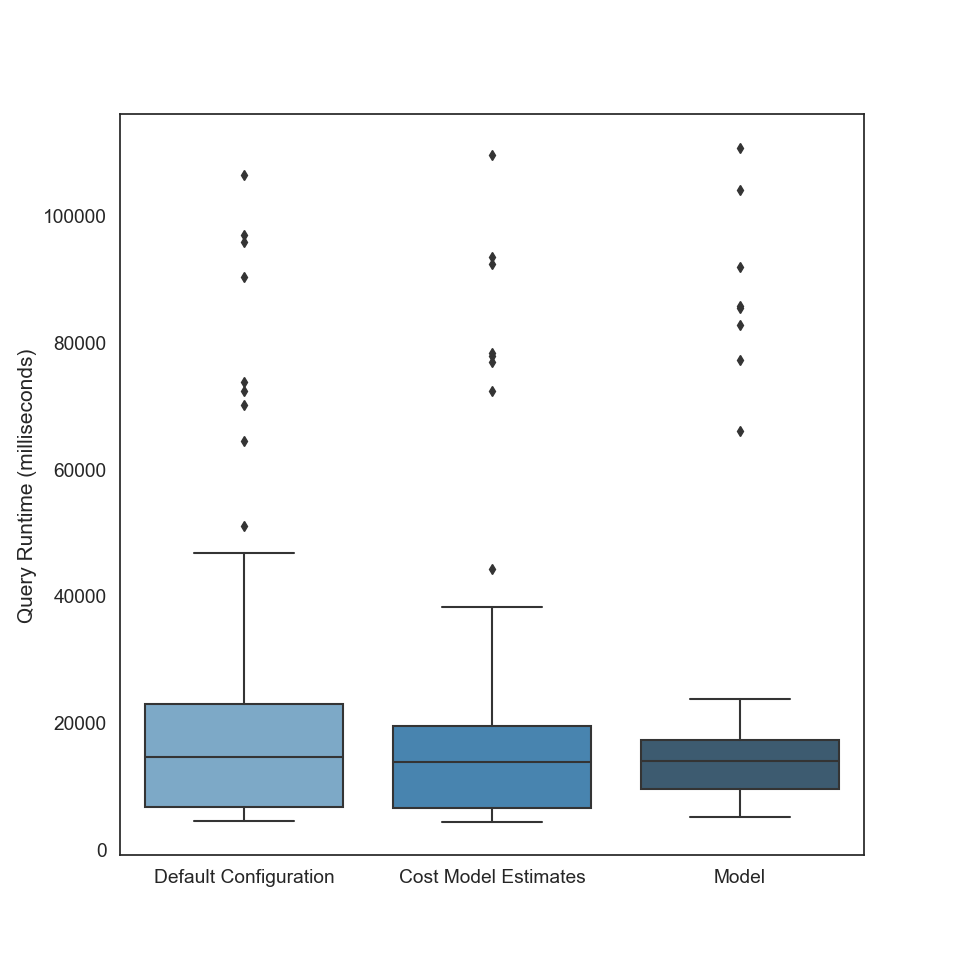
\includegraphics[width=\textwidth]{img/performance_evaluation/tpch_rf_optimizer_comparison.png}
    \caption{\gls{tpch} workload}
    \label{fig:tpch_boxplot}
    \end{subfigure}\hfill
    \begin{subfigure}[t]{0.5\textwidth}
    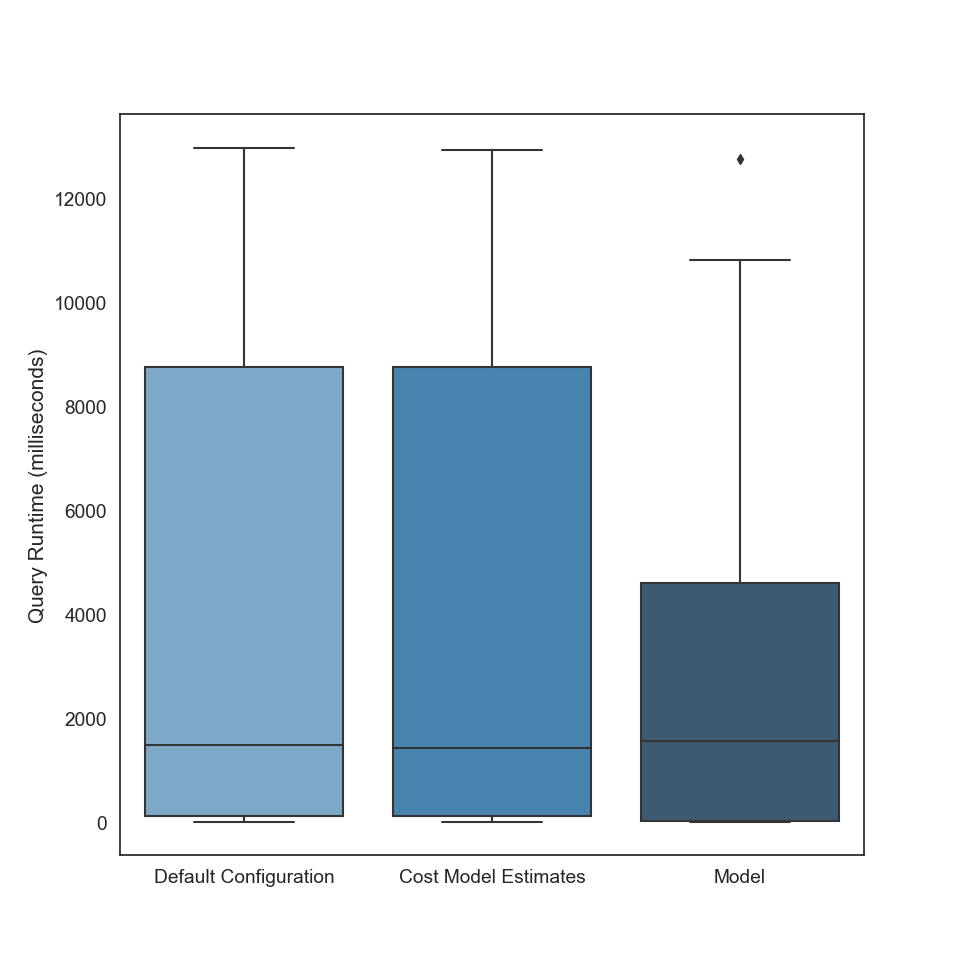
\includegraphics[width=\textwidth]{img/performance_evaluation/job_rf_optimizer_comparison.png}
    \caption{\gls{job} workload}
    \label{fig:job_boxplot}
    \end{subfigure}
    \caption{Query runtime comparison between the three approaches} 
    \label{fig:boxplot}
\end{figure}

Figure \ref{fig:boxplot} summarizes the results using the three different approaches. Using cost model estimates for the \gls{tpch} queries resulted in a slight improvement over the default configuration, but the learned model still outperformed both. On the other hand, for the \gls{job} queries, using the cost model estimates and leaving the optimizer settings to the default configuration, resulted in nearly the same execution runtime distribution, whereas the learned approach surpassed both.

\subsubsection{Operator Type Analysis}

Evaluating the proposed solution on a query-level basis allowed to delve into the model's optimizer settings configuration choices. Throughout the experimental evaluation, the chosen configuration for each one of the assessed queries was recorded. As a result, it is possible to infer the number of times a given operator type was selected to be disabled and discover specific patterns between the two workloads. It is important to note that the choice of operators is not mutually exclusive, meaning that a given configuration may simultaneously include two or more operators.

\begin{figure}[H]
\begin{subfigure}[t]{\textwidth}
    \centering
    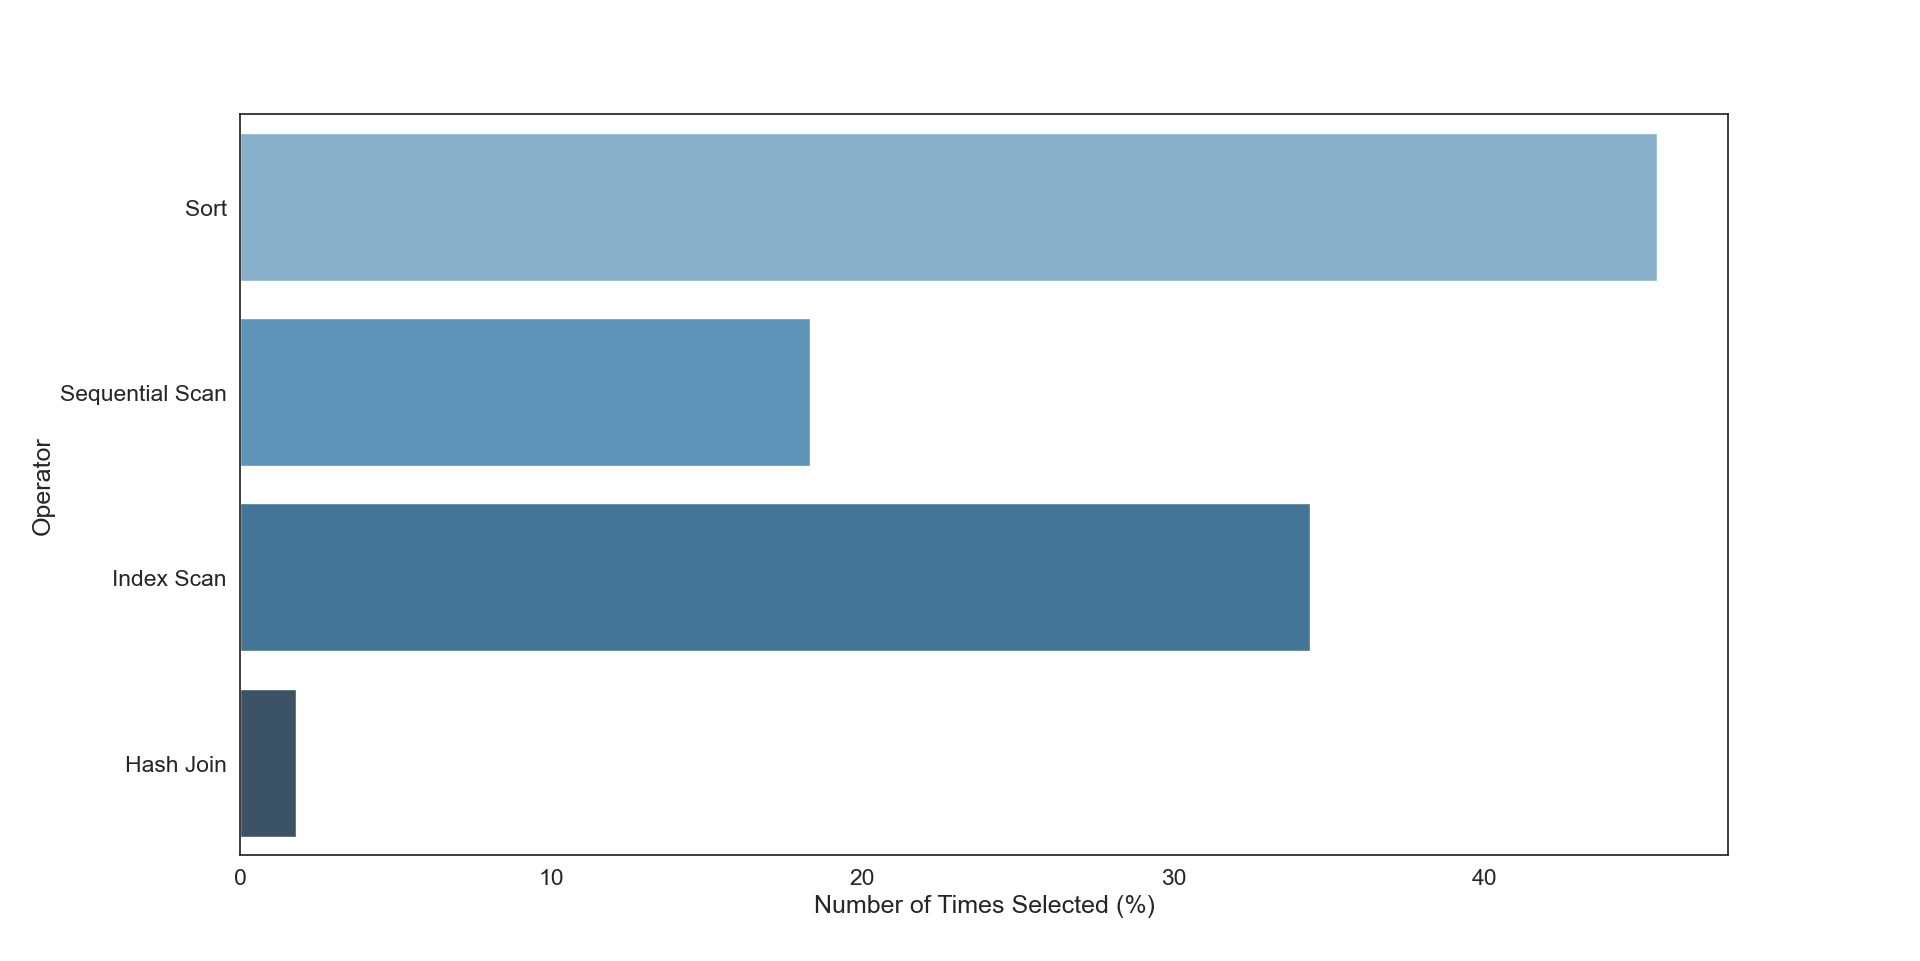
\includegraphics[width=0.8\textwidth]{img/performance_evaluation/tpch_operator_analysis.png}
    \caption{\gls{tpch} workload}
    \label{fig:tpch_operator_analysis}
\end{subfigure}
\begin{subfigure}[t]{\textwidth}
    \centering
    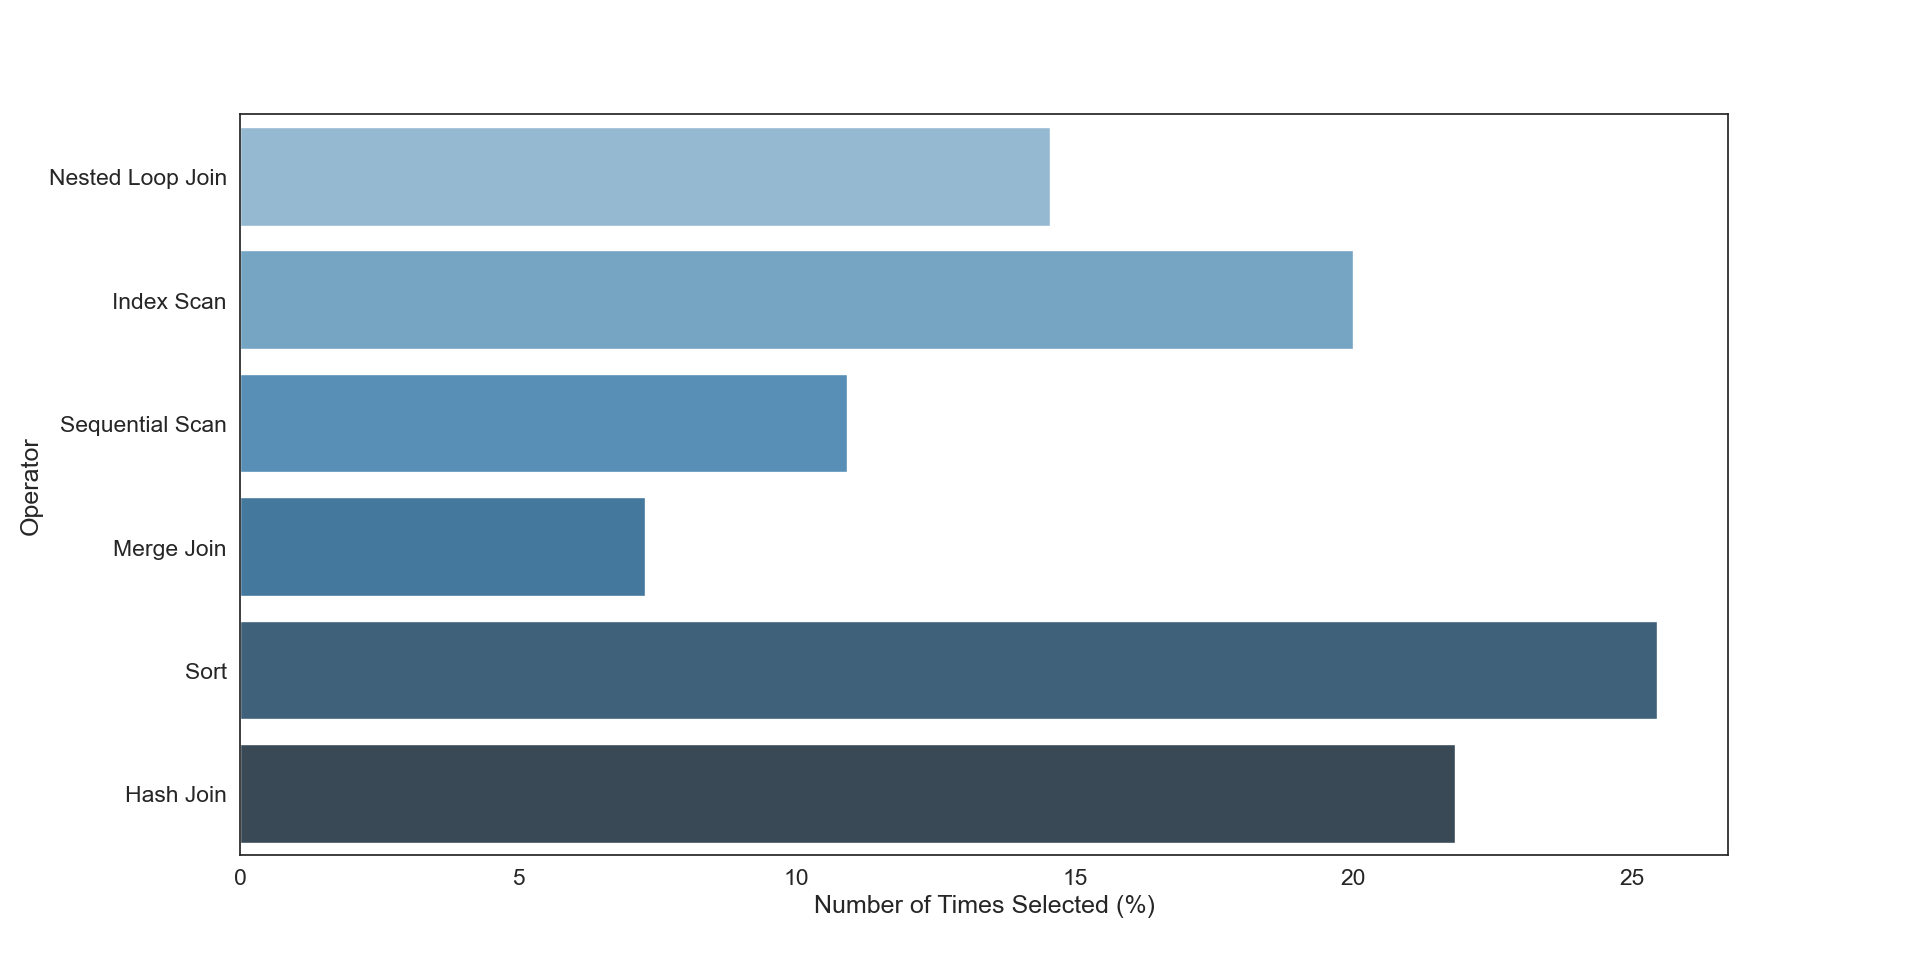
\includegraphics[width=0.8\textwidth]{img/performance_evaluation/job_operator_analysis.png}
    \caption{\gls{job} workload}
    \label{fig:job_operator_analysis}
\end{subfigure}
\caption{Number of times an operator was selected to be disabled}

\end{figure}

Figure \ref{fig:tpch_operator_analysis} shows that only four operator types are dismissed throughout the experimental evaluation for the \gls{tpch} workload, with the \textit{sort} being the most frequent one. The choice of disabling the \textit{index scan} could be explained by the absence of indices, while \textit{sequential scan} tends to be one of the most costing types of operations. Bear in mind that disabling each of these operators does not necessarily mean that it was the right decision, as there are some cases where performance regressions happen.

Similar to the previous one, Figure \ref{fig:job_operator_analysis} illustrates which types of operators are discarded throughout the experiments for the \gls{job} workload. Notice how two additional join operator types are now considered compared to the \gls{tpch} workload. It can be easily explained by the fact the most of the \gls{job} queries have an average of 8 joins per query, as mentioned before.

\subsubsection{Query Type Analysis}

This section evaluates the difference in performance relative to the default set of settings for each query. To get more insight about which type of queries can benefit the most by using machine learning, the query performance for each of the executed \gls{tpch} queries in the experimental phase was analyzed.

\begin{figure}[H]
\centering
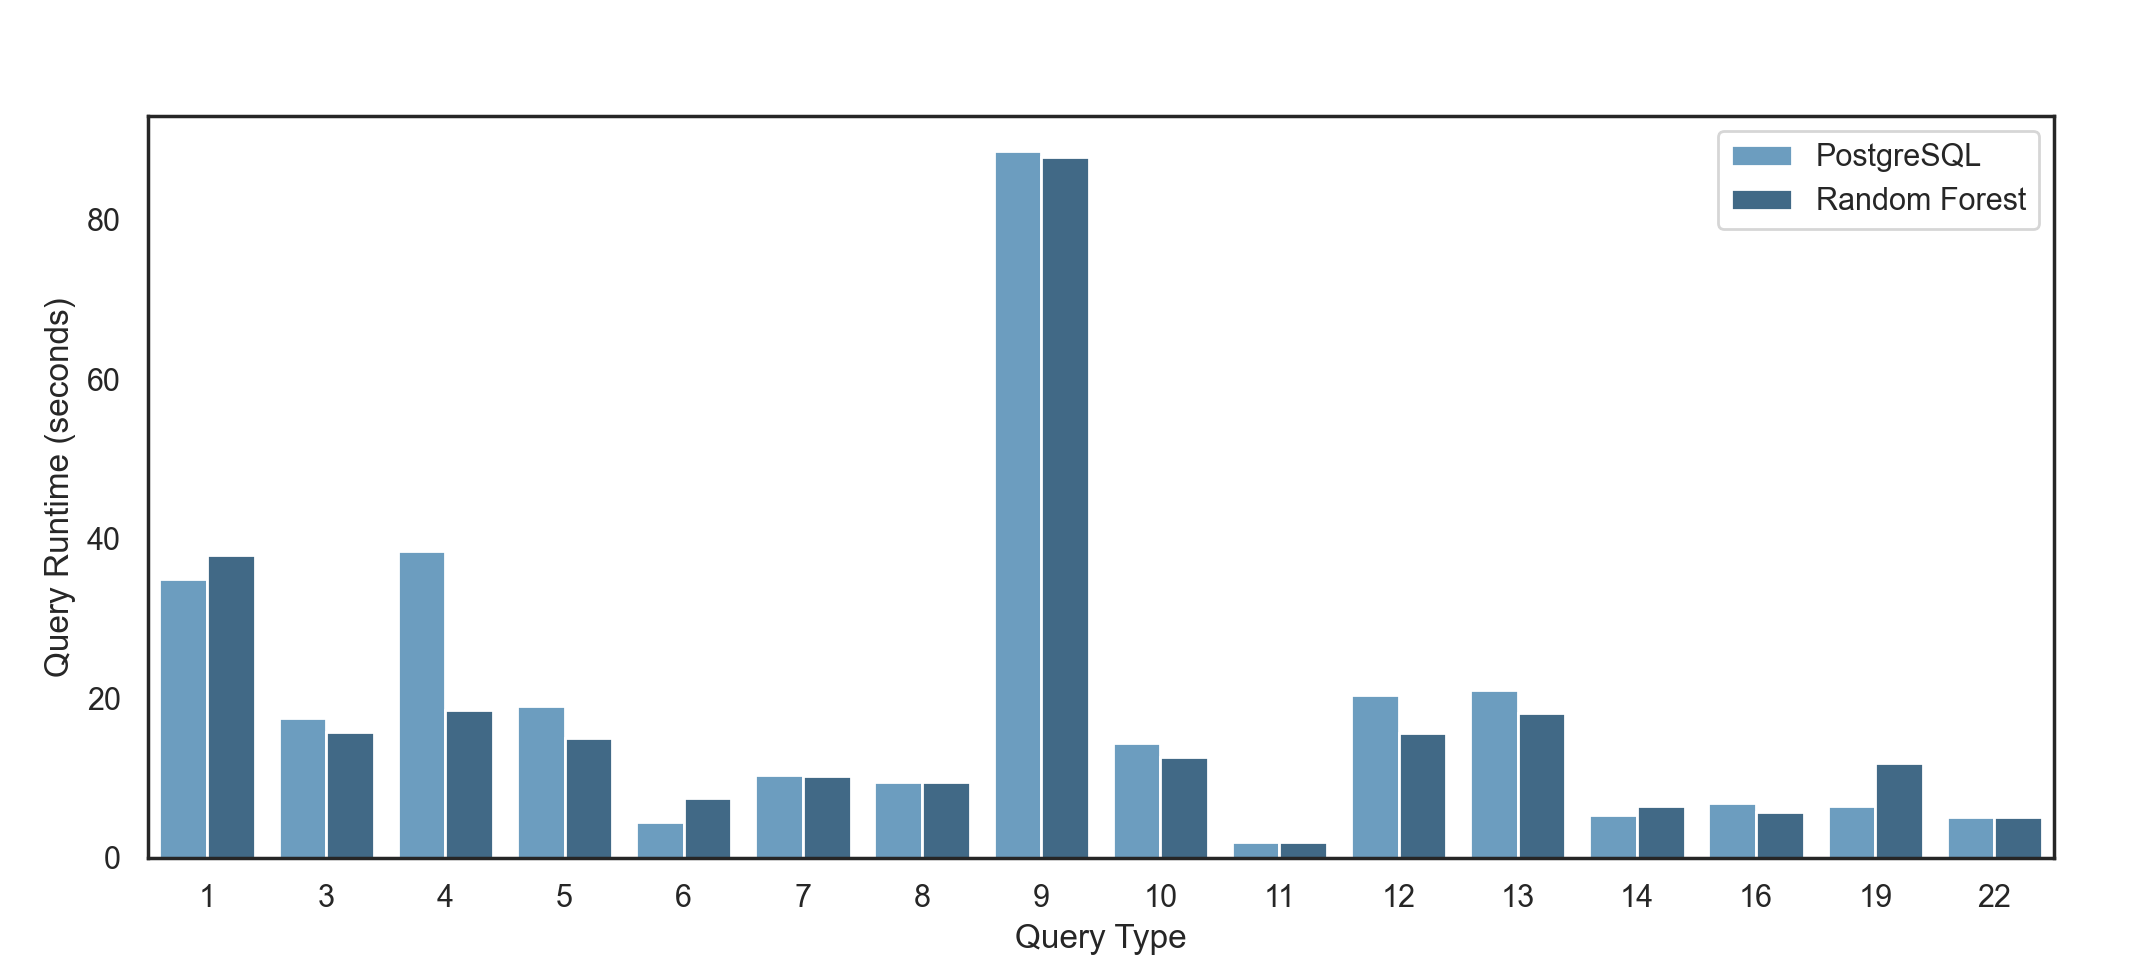
\includegraphics[width=\textwidth]{img/performance_evaluation/tpch_query_analysis.png}
\caption{Runtime difference per query between PostgreSQL and Random Forest for the \gls{tpch} workload}
\label{fig:tpch_query_analysis}
\end{figure}

Figure \ref{fig:tpch_query_analysis} shows the difference in runtime between the plan chosen by our learned approach and the PostgreSQL default one. Of the 16 \gls{tpch} queries shown above, the Random Forest algorithm only incurs regressions on five, and these regressions are all under 5 seconds. The remaining 11 see performance improvements of up to 20 seconds. While the learned algorithm does not always choose the best plan compared to the default configuration, it comes close to almost every query.

Please note that a specific threshold was enforced to avoid unwanted significant query performance regressions, set to 0.15 by default. Increasing the regression threshold would help to decrease the probability of such regressions at the cost of decreasing the probability of potential query performance improvements.

\subsection{Inference and Training Overhead}

A significant concern with any application of machine learning is training time overhead. Across all workloads, generating the data set is the procedure that takes longer since it requires that a single query run multiple times with different configurations to make the training process more robust. As a result, the training process will better capture the impact of different settings on the final query execution runtime.

For the \gls{tpch} workload:

\begin{itemize}
    \item Generating the data set takes about 16.4 hours, using ten queries per template;
    \item Training the model takes up to 12 seconds;
    \item Inferring the best plan had a maximum increase of 114 milliseconds on planning time compared to the out-of-the-box PostgreSQL optimizer.
\end{itemize}

As for the Join Order Benchmark:

\begin{itemize}
    \item Generating the data set takes about 25 minutes;
    \item Training the model takes up to 13 seconds;
    \item Inferring the best plan had a maximum increase of 613 milliseconds on planning time compared to the out-of-the-box PostgreSQL optimizer.
\end{itemize}

Since analytic queries generally run for many seconds or minutes, an optimization time of a few milliseconds may be acceptable in most applications. Seeing that generating the data set may take up much time, even for a relatively small data set, this work further proposes new considerations that could be taken into account when applying machine learning-based query optimization solutions in a real-world scenario.

\subsection{Translating Into a Real-World Scenario}

Most machine learning algorithms focus on batch training, meaning that all training data is available beforehand. More recent techniques allow the training process to be done incrementally while a continuous stream of data is made available over time. Stream learning models are created incrementally and are updated continuously. Learning incrementally from a mini-batch of instances would be essential to out-of-core learning in query optimization. It would take away the concern of having queries execution history.

In a real-world scenario, changes in data distribution may harm learning. Using an adaptive sliding window method would allow the algorithms to be more robust to concept drift changes in dynamic environments such as query optimization. The general idea is to keep metrics and statistics from a window of variable size. The algorithm decides the window's size by cutting the window at different points and analyzing the average of a particular metric over these two windows. If the difference between the two averages surpasses a pre-defined threshold, change is detected, and all data before that time is discarded.

In the context of stream learning, another concern is evaluating the performance of a learned model. It can be measured using two predominant techniques:

\begin{itemize}
    \item Using a holdout evaluation where the performance evaluation happens periodically, at which moment the evaluator will test the learner's performance on a test set, formed by yet unseen queries, which will be used to evaluate performance, but not to train the model;
    \item Using a prequential evaluation where each data sample serves two purposes. Each query is analyzed sequentially, in order of arrival, and becomes immediately inaccessible. This method involves using each sample to test the model (i.e., make a prediction) and then use the same sample to train the model. By doing this, the model is always tested on samples that it has not seen yet.
\end{itemize}

Being conceived to serve as a platform to encourage the democratization of stream learning research, \textit{scikit-multiflow} \citep{montiel2018} is a framework that provides multiple state-of-the-art learning methods, data generators, and evaluators for different stream learning problems. It builds upon popular open-source frameworks, including \textit{scikit-learn} \citep{pedregosa2011}, in which our solution is built upon.